\chapter*{Введение}\label{Input}
\addcontentsline{toc}{chapter}{Введение}

\textbf{Расстояние Левенштейна} -- это минимальное количество редакторских операций необходимое для 
превращения одной строки в другую. Редакторскими операциями считаются вставка, удаление, замена.

Расстояние Дамерау-Левенштейна включает также операцию перестановки 2 символов.

Расстояние Левенштейна применяется в следующих сферах:
\begin{itemize}
  \item компьютерная лингвистика:
  \begin{itemize}
    \item автозамена;
    \item сравнение текстов;
    \item поисковые системы;
  \end{itemize}
  \item биоинформатика:
  \begin{itemize}
    \item сравнение генов, хромосом и белков.
  \end{itemize}
\end{itemize}


Целью данной лабораторной являются изучение метода динамического программирования на материале алгоритмов Левенштейна и Дамерау-Левенштейна.
Задачами данной лабораторной являются:
\begin{enumerate}
  \item изучение алгоритмов Левейнштейна и Дамерау-Левенштейна нахождения расстояния между строками;
  \item применение метода динамического программирования для матричных алгоритмов;
  \item реализация указанных алгоритмов;
  \item сравнительный анализ линейной и рекурсивной реализаций выбранного алгоритма определения расстояния между строками по затрачиваемым 
        ресурсам(времени и памяти);
  \item экспериментальное подтверждение различий во временной эффективности рекурсивной и нерекурсивной реализаций выбранного алгоритма 
        определения расстояния между строками при помощи разработанного времени выполнени7я реализации на варьирующихся длинах строк;
  \item описание и обоснование полученных результатов в отчете о выполненной лабораторной работе, выполненного как расчетно-пояснительная 
        записка к работе.
\end{enumerate}

\chapter{Аналитическая часть}\label{Analis}
%\addcontentsline{toc}{chapter}{1 Аналитическая часть}

Для поиска расстояний между строками необходимо определить расстояние между строками и разработать алгоритм, его нахождения.

\section{Описание проблемы поиска расстояния Левенштейна}\label{LeventsheinProblem}

\textbf{Расстояние Левенштейна} -- это минимальное количество редакторских операций необходимое для 
превращения одной строки в другую. \cite{levenshtein} Редакторскими операциями считаются: %(\cite{litlink1})
\begin{enumerate}
  \item вставка(I - insert), 
  \item удаление (D - delete), 
  \item замена (R - replace).
\end{enumerate}
Совпадение помечается буквой M - merge.
\\

Найти расстояние Левенштейна можно тремя способами:
\begin{enumerate}
  \item матрично;
  \item рекурсивно;
  \item рекурсивно с кэшем.
\end{enumerate}

На рисунке \ref{ris:levenshtein_example} показан пример расчета расстояния Левенштейна.

\begin{figure}[H]
  \center{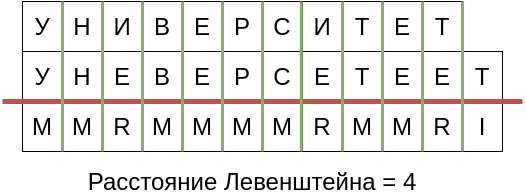
\includegraphics[scale=0.5]{l1.levenshtein}}
  \caption{Пример расчета расстояния Левенштейна}
  \label{ris:levenshtein_example}
\end{figure}


\section{Рекурсивный алгоритм поиска расстояния Левенштейна}\label{RecursiveLeventshein}

Алгоритм можно описать следующей формулой $d(S_1, S_2) = D(M,N)$, где $S_1$ и $S_2$ - две строки длиной М и N над некоторым алфавитом. 


\begin{equation*}
  D = 
  \begin{cases}
    max(i,j), &\text{i = 0 or j = 0}\\
    min\{ \\
      ~~~~D(i,j-1)+1,\\
      ~~~~D(i-1,j)+1, &\text{i > 0, j > 0}\\
      ~~~~D(i-1,j-1)+m(S_1[i],S_2[j])\\
    \}
    \end{cases}
\end{equation*}

где $m(a,b) = 0$, если $a=b$, иначе $m(a,b) = 1$, $min(a,b,c)$ - возвращает наименьший аргумент, 
$max(a,b,c)$ - возвращает набольший аргумент

\section{Рекурсивный алгоритм поиска расстояния Левенштейна с кешем}\label{RecursiveKeshLeventshein}

В рекурсином алгоритме часто повторяются одинаковые действия, т.к. не храняться уже вычисленные значения. 
Проблема показана на рисунке \ref{ris:problem_levenshtein_example}. На рисунке красным выделены итерации, 
которые выполняются несколько раз, что требует дополнительные вычисления.


\begin{figure}[H]
  \center{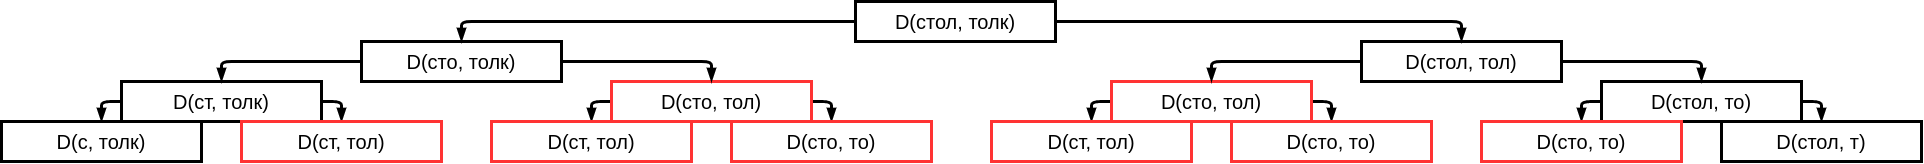
\includegraphics[scale=0.25]{l1.levenshteinrecursiveproblema.png}}
  \caption{Проблема рекурсивного метода}
  \label{ris:problem_levenshtein_example}
\end{figure}

Для решения этой проблемы можно использовать кеширование. Необходимо запоминать строки, над которыми выполняется операция, и ее результат.
Способ, использующий кеш, называется рекурсивный алгоритм поиска расстояния Левенштейна с кешем.

\section{Матричный алгоритм поиска расстояния Левенштейна}\label{MatrixLeventshein}

На рисунке \ref{ris:matrix_example} показан пример расчета расстояния Левенштейна матричным способом.

\begin{figure}[H]
  \center{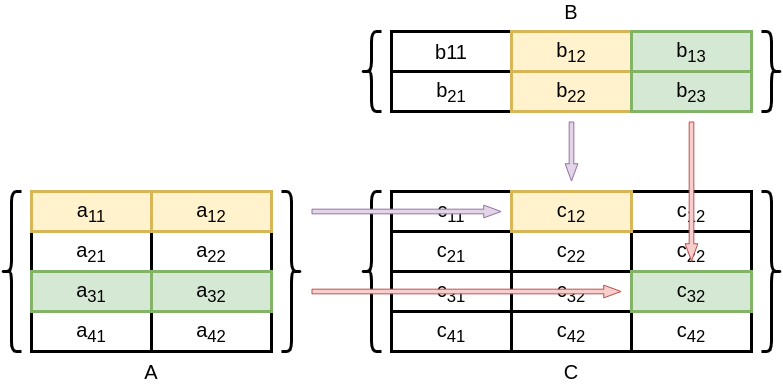
\includegraphics[scale=0.5]{l1.matrix}}
  \caption{Пример расчета расстояния Левенштейна матричным способом}
  \label{ris:matrix_example}
\end{figure}

На рисунке \ref{ris:recurs_example} показан пример расчета расстояния Левенштейна матричным способом.

\begin{figure}[H]
  \center{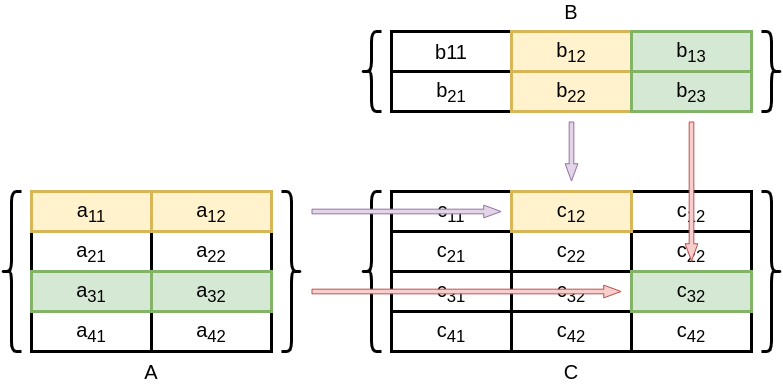
\includegraphics[scale=0.5]{l1.matrix}}
  \caption{Пример расчета расстояния Левенштейна матричным способом}
  \label{ris:recurs_example}
\end{figure}

\section{Рекурсивный алгоритм поиска расстояния Дамерау - Левенштейна}\label{Dameray_Leventshein}

\textbf{Расстояние Дамерау-Левенштейна} -- это минимальное количество редакторских операций необходимое для 
превращения одной строки в другую. Редакторскими операциями считаются:
\begin{enumerate}
  \item вставка(I - insert), 
  \item удаление (D - delete), 
  \item замена (R - replace),
  \item перестановка 2 соседних символов (X - change).
\end{enumerate}
Совпадение помечается буквой M - merge.

Расстояние Дамерау-Левенштейна в некоторых случаях может быть короче расстояния Левенштейна. (рис. \ref{ris:dameray_levenshtein_example}).

\begin{figure}[H]
  \center{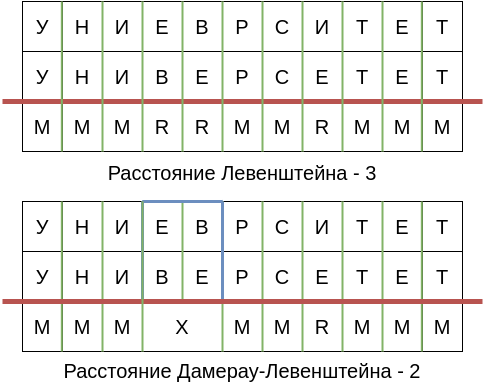
\includegraphics[scale=0.5]{l1.dameray-levenshtein}}
  \caption{Сравнение расчета расстояний Левенштейна и Дамерау-Левенштейна}
  \label{ris:dameray_levenshtein_example}
\end{figure}


Алгоритм можно описать следующей формулой, где $S_1$ и $S_2$ - две строки длиной М и N над некоторым алфавитом. 
Тогда расстояние Дамеау-Левенштейна $d(S_1, S_2) = D(M,N)$.

\begin{equation*}
  D = 
  \begin{cases}
    max(i,j), &\text{i = 0 or j = 0}\\
    min\{ \\
      ~~~~D(i,j-1)+1,\\
      ~~~~D(i-1,j)+1, &\text{i > 1, j > 1 and $a_i$ = $b_{j-1},a_{i-1}$ = $b_j$}\\
      ~~~~D(i-1,j-1)+m(S_1[i],S_2[j]),\\
      ~~~~D(i-2,j-2)+1\\
    \},\\
    min\{ \\
      ~~~~D(i,j-1)+1,\\
      ~~~~D(i-1,j)+1, &\text{other}\\
      ~~~~D(i-1,j-1)+m(S_1[i],S_2[j])\\
    \}
    \end{cases}
\end{equation*}

где $m(a,b) = 0$, если $a=b$, иначе $m(a,b) = 1$, $min(a,b,c)$ - возвращает наименьший аргумент, 
$max(a,b,c)$ - возвращает набольший аргумент.


\section{Вывод аналитической части}\label{End_analis_chapter}

В данной работе стоит задача реализации следующих алгоритмов поиска расстояния Левенштейна: матричный алгоритм, рекурсивный алгоритм и 
рекурсивный алгоритм с кешем, и задача реализации рекурсивного алгоритма поиска расстояния Дамерау-Левенштейна. Необходимо сравнить 
алгоритмы поиска расстояния Левенштейна по эффективности по времени и памяти.

Реализуем алгоритмы и сравним их затраченные на их выполнение время и память.
 

